\documentclass{article}
\usepackage[top=1in,left=1in,bottom=1in,right=1in]{geometry}
\usepackage{float}
\usepackage{graphicx}
\usepackage{amsmath}
\usepackage{xcolor}
\usepackage{booktabs}

\begin{document}

\begin{centering}
  NE/MP 506\\
  Practicum in Monte Carlo Radiation Transport\\
  Exam \#1 - Spring 2024\\
\end{centering}

\vspace*{0.2in}

\textbf{Random Numbers:} Random Numbers: For each question use the following
random numbers.  There may be more random numbers than you need for each
question.  If there are not enough random numbers start using the numbers for
the next question

\begin{center}
\begin{tabular}{|c|c|c|c|c|c|c|}
  \hline
Q1 & 0.886598 & 0.856192 & 0.752546 & 0.367955 & 0.611161 & 0.483739\\ \hline

Q2 & 0.618436 & 0.845987 & 0.205497 & 0.429765 & 0.962275 & 0.232004 \\ \hline

Q3 & 0.610944 & 0.795906 & 0.029646 & 0.115320 & 0.150826 & 0.499478 \\ \hline

Q5 & 0.670521 & 0.490479 & 0.443408 & 0.808839 & 0.536873 & 0.477459 \\ \hline
\end{tabular}
\end{center}

\begin{enumerate}
\item A volume source is described by the following three distributions in x, y, and z.

In the x-direction, the source is distributed with the form:

  $$p(x) = x^2,\ \ \ 0\ cm < x < 25\ cm.$$


In the y-direction, it follows the distribution shown in the figure below.

  \begin{center}
      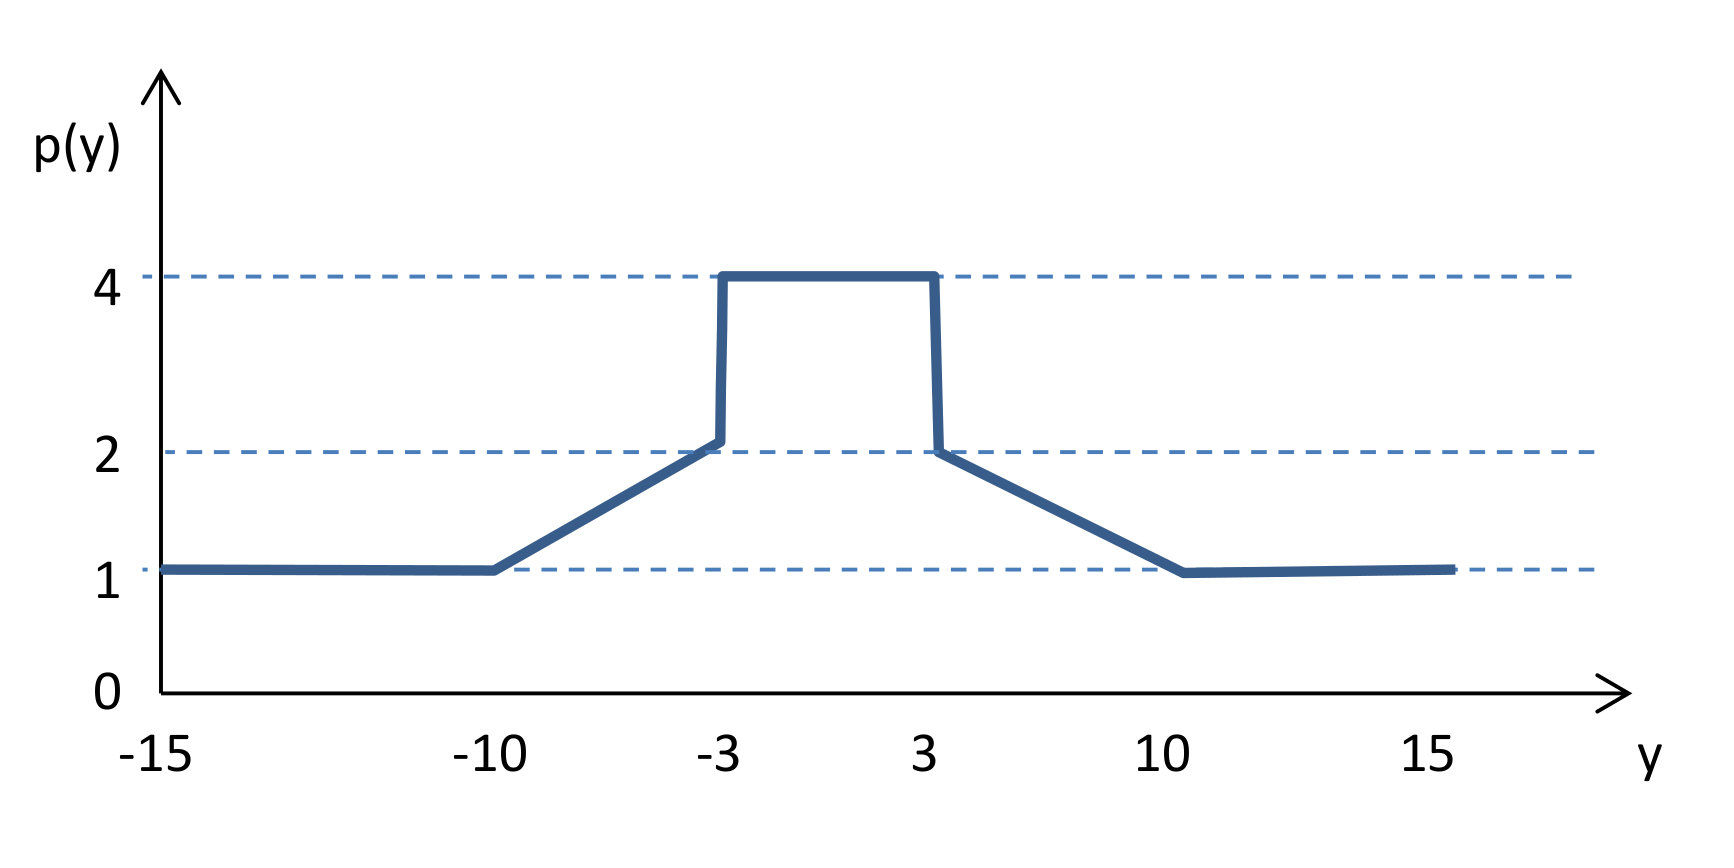
\includegraphics[width=3.5in]{piecewise-linear-y.png}
  \end{center}

In the z-direction, the source is uniformly distributed
between $0\ cm$ and $25\ cm$.

  \begin{enumerate}
  \item Sample the source position in the x-direction

  \item Sample the source position in the y-direction

  \item Sample the source position in the z-direction
  \end{enumerate}

  \newpage

\item The energy of the source is described by the following distribution.
  Sample the initial energy of a particle from this source.

  $$PDF:\ f(E) = sin(\frac{7E}{\pi})^{2}cos(\frac{15E}{\pi})^{2}\ , \ 0 \leq E \leq 10 MeV $$

  \begin{center}
      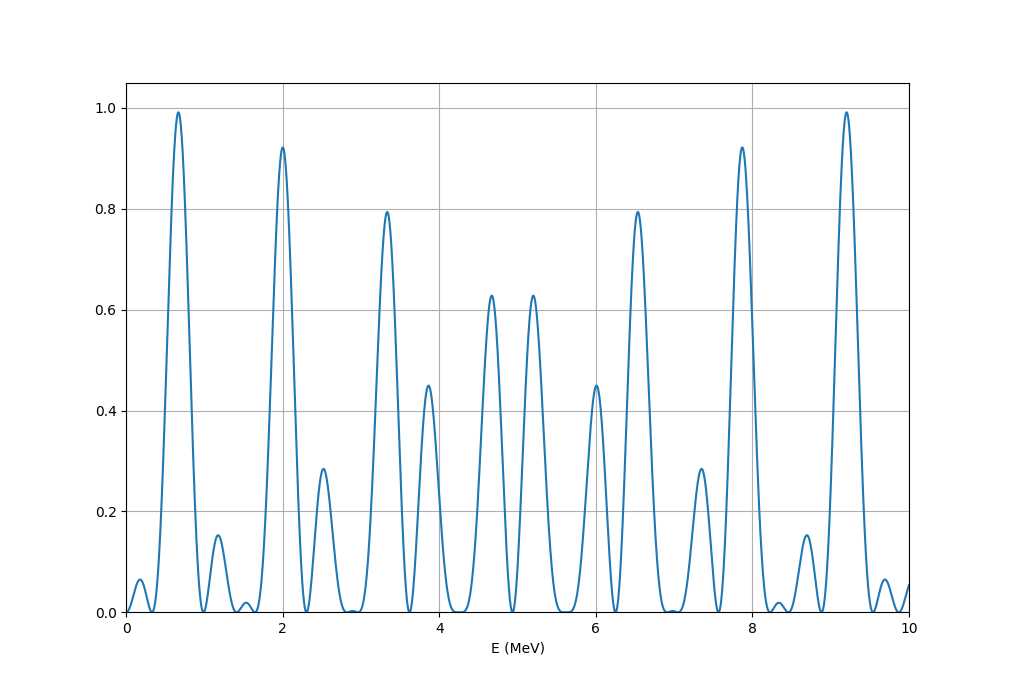
\includegraphics[width=4.5in]{energy-dist.png}
  \end{center}

  \newpage

\item The geometry of this problem involves a sphere of water, centered at (1, 5, 4) with a radius of 10 cm.
Two cylinders (radii of 2.5 cm) parallel to the z axis are removed from the sphere (see figure below).
The cylinders are centered at (-9, 5, 4) and (11, 5, 4). The source position is (1, 1, 4). A particle is
born with direction (0.8242, 0.5494, -0.1374). If the particle does not collide in the material, where will
it leave the cell? Check all surfaces where a boundary crossing could possibly occur.


\begin{center}
  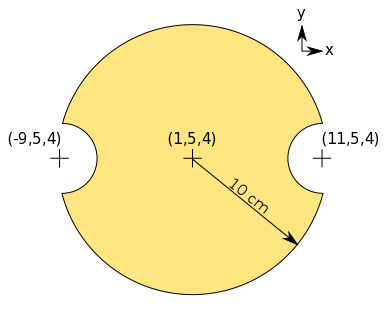
\includegraphics[width=2.5in]{exam1-analytic-geom.png}
\end{center}


\item If the total attenuation coefficient of the water is $0.78 cm^{-1}$,
  where will the first collision occur for a particle with starting conditions
  given in problem 4?

\end{enumerate}



\end{document}
